\documentclass[12pt,a4paper]{article}
\usepackage[top=2cm,bottom=2cm,left=2cm,right=1.5cm]{geometry}
\usepackage[utf8]{vietnam}
\usepackage{tikz}
\begin{document}
	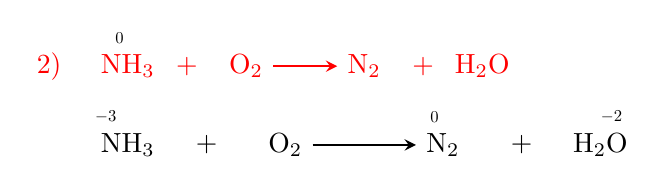
\begin{tikzpicture}[>=stealth,thick]
		\path
		(-1,0) node[red]{$2)$}
		(0,0) node[red]{$\mathrm{NH_3}$}
		(.75,0) node[red]{+}
		(1.5,0) node[red](A){$\mathrm{O}_2$}
		(3,0) node[red](B){$\mathrm{N_2}$}
		(3.75,0) node[red]{+}
		(4.5,0) node[red]{$\mathrm{H_2O}$}
		(0,-1) node{$\mathrm{NH_3}$}
		+(-8pt,10pt) node[scale=.6]{$-3$}
		(1,-1) node{+}
		(2,-1) node(C){$\mathrm{O}_2$}
		(-3pt,10pt) node[scale=.6]{$0$}
		(4,-1) node(D){$\mathrm{N_2}$}
		+(-3pt,10pt) node[scale=.6]{$0$}
		(5,-1) node{+}
		(6,-1) node{$\mathrm{H_2O}$}
		+(4pt,10pt) node[scale=.6]{$-2$};
		\draw [->,red] (A)--(B);
		\draw [->] (C)--(D);
	\end{tikzpicture}
	Với $\mathrm{NH_3}$ là chất khử, $ \mathrm{O_2} $ là chất oxi hóa.
	\begin{tikzpicture}[>=stealth,thick]
		\path
		(0,0) node{$6 \ \times \ $}
		(1,0) node{$\mathrm{O_2}$}
		+(-3pt,10pt) node[scale=.6]{$0$}
		(1.75,0)node{+}
		(3,0) node (A) {$2 \times 2 \mathrm{e}$}
		(5,0) node (B) {$2\mathrm{O}$}
		+(3pt,10pt) node[scale=.6]{$-2$}
		(7,0) node[right]{(quá trình khử)}
		(0,-1) node{$4 \ \times \ $}
		(1,-1) node{$\textcolor{red}{2}\mathrm{N}$}
		+(3pt,10pt) node[scale=.6]{$-3$}
		(1.75,-1) node{+}
		(3,-1) node (C) {$\textcolor{red}{2} \times 3 \mathrm{e}$}
		(4.75,-1) node(D){$\textcolor{red}{2}\mathrm{N}$}
		+(3pt,10pt) node[scale=.6]{$0$}
		(6,-1) node{$ \mathrm{(N_2)} $}
		(7,-1) node[right]{(quá trình oxi hóa)}
		(0,-2) node{$4\mathrm{NH_3}$}
		(1,-2) node{+}
		(2,-2) node (E) {$3\mathrm{O}_2$}
		(4,-2) node (F) {$2\mathrm{N_2}$}
		(5,-2) node{+}
		(6,-2) node{$6\mathrm{H_2O}$};
		\draw (.4,.5)--(.4,-1.4);
		\draw[very thick, red](-.5,-1.5)--(6.5,-1.5);
		\draw[->] (A)--(B);
		\draw[->] (C)--(D);
		\draw[->] (E)--(F);
	\end{tikzpicture}
\end{document}